% 
% Interface
% @author Pieter Maene <pieter.maene@student.kuleuven.be>
%

\chapter{Interface}
\label{chap:interface}

Het verbeteren van de gebruiksvriendelijkheid van het Helios verkiezingssysteem was een belangrijk doel van deze thesis. Er zijn op vier belangrijke plaatsen wijzigingen aangebracht. Veruit het meeste werk was nodig om de procedure van \ref{chap:procedure} duidelijker te maken in het beheer (\ref{sec:ui:beheer}). Ook de gebruiksvriendelijkheid van het trustee dashboard werd sterk verbeterd (\ref{sec:ui:trustee_dashboard}). Tot slot werd ook de output van de applicatie die gebruikt kan worden om het resultaat te controleren, verduidelijkt (\ref{sec:ui:controleapplicatie}). Hoewel in dit hoofdstuk alleen de grootste aanpassingen besproken worden, werd de layout doorheen het hele systeem geüniformeerd.

\section{Beheer}
\label{sec:ui:beheer}

In de oude interface zaten het beheer en het bekijken van de verkiezing op dezelfde pagina (\ref{fig:ui:elections_view_old}). De gewone kiezers zagen de beheersfuncties uiteraard niet, maar dit maakte het wel ingewikkeld voor de beheerder. Bovendien was het niet duidelijk wat de volgende stap was of waar de beheerder juist in de procedure zat. Daarom werd besloten om deze twee functies uit elkaar te halen en een aparte pagina te voorzien voor het beheer (\ref{fig:ui:elections_admin}).

\begin{figure}
  \center{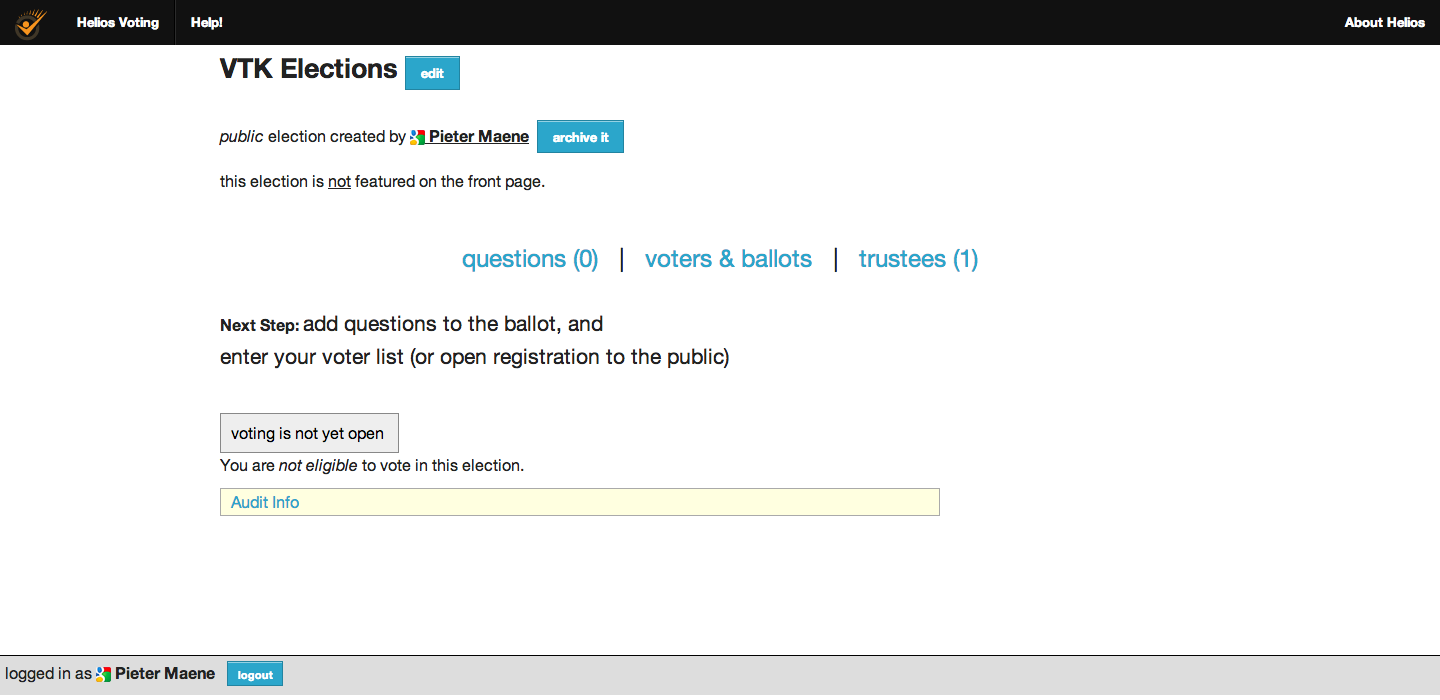
\includegraphics[width=\linewidth]{ui/elections_view_old.png}}
  \caption{Overzicht van de verkiezing (oud)}
  \label{fig:ui:elections_view_old}
\end{figure}

\begin{figure}
  \center{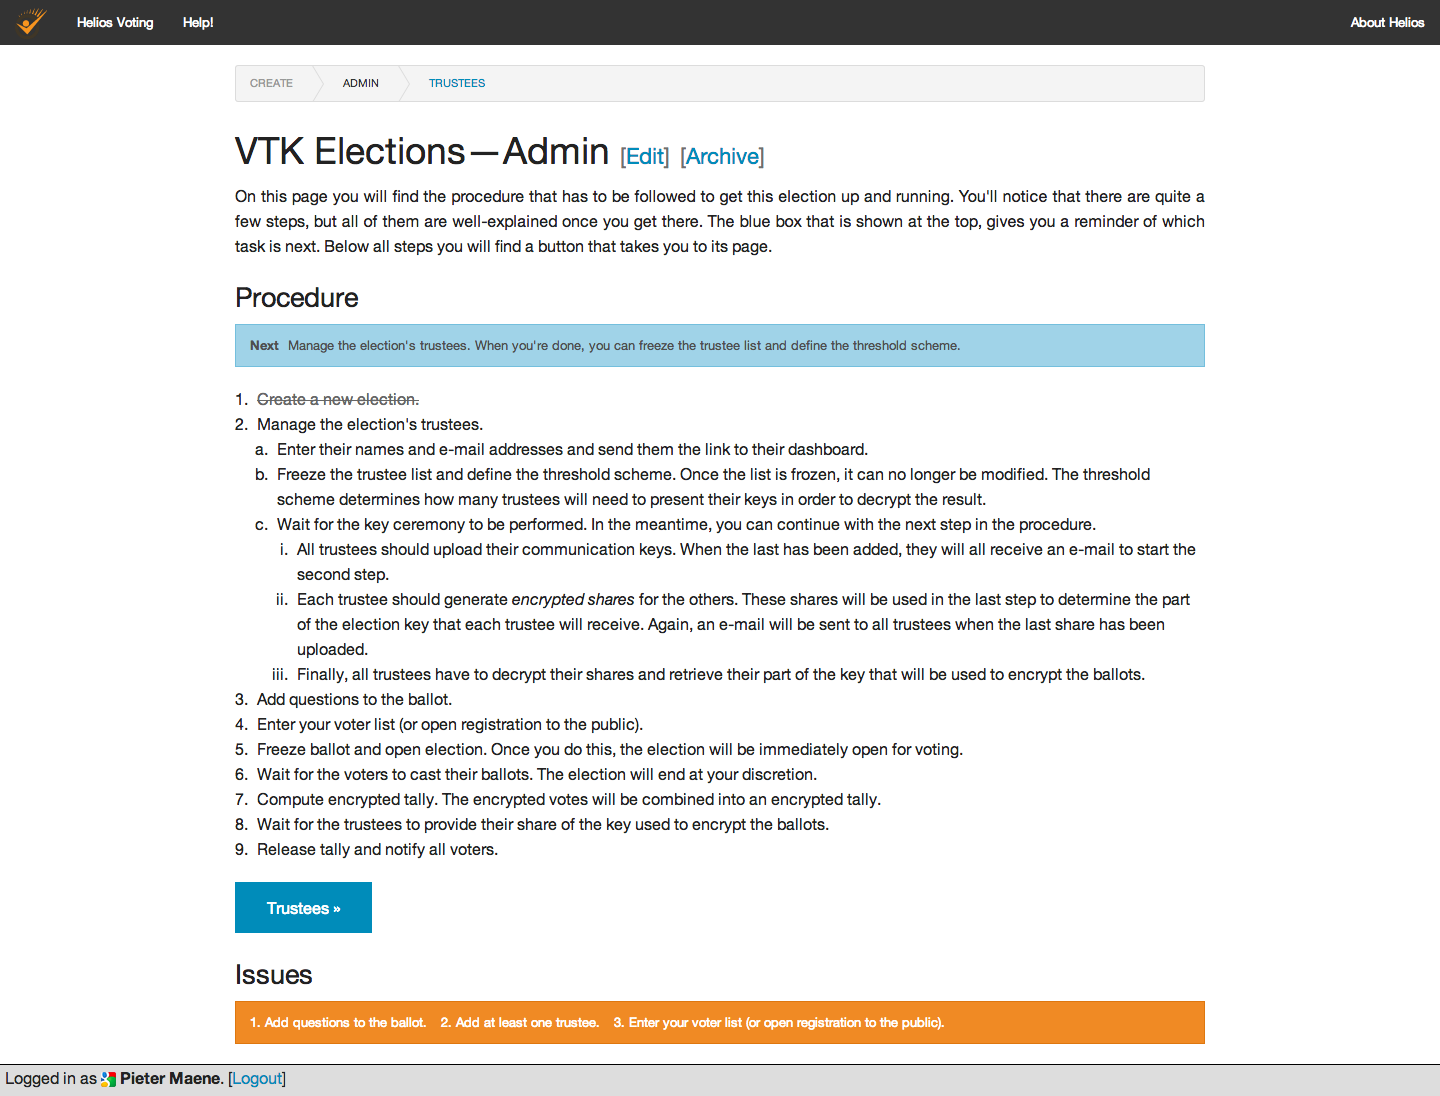
\includegraphics[width=\linewidth]{ui/elections_admin.png}}
  \caption{Beheer van de verkiezing}
  \label{fig:ui:elections_admin}
\end{figure}

\npar Op deze nieuwe pagina wordt de volledige procedure weergegeven. Er wordt ook aangegeven wat de volgende stap is en welke stappen reeds allemaal voltooid zijn. Tot slot staan onderaan alle problemen die nog opgelost moeten worden voordat het stembiljet bevroren kan worden. Bovendien wordt bovenaan elke pagina ook getoond waar hij zit en wat de volgende stap is (\ref{fig:ui:election_progress}). Zo kan hij dit ook volgen wanneer hij niet op de speciale beheerpagina zit.

\begin{figure}
  \center{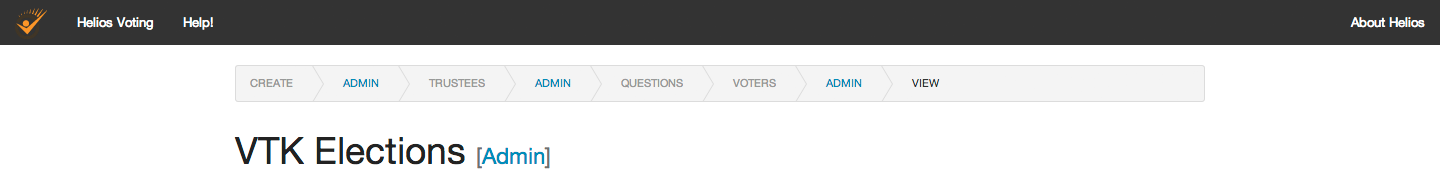
\includegraphics[width=\linewidth]{ui/election_progress.png}}
  \caption{Voortgang procedure}
  \label{fig:ui:election_progress}
\end{figure}

\npar Voor een verkiezing met threshold encryptie (\ref{sec:helios:threshold_encryptie}) zijn er belangrijke veranderingen in de workflow. Robbert Coeckelbergh had een publiek bulletin board ge\"introduceerd waar iedereen sleutelparen voor communicatie kon aanmaken en uploaden. De beheerder kon dan trustees toevoegen aan een verkiezing door ze te selecteren uit een lijst. Dit betekent ook dat dezelfde sleutelparen voor communicatie gebruikt werden bij elke verkiezing waar deze persoon trustee was.

\npar Voordat alle trustees toegevoegd konden worden aan een trustee, moest de beheerder dus wachten totdat iedereen zijn sleutelparen voor communicatie ge\"upload had. Omdat iedereen hiervoor buiten het systeem om nog eens gecontacteerd moest worden, maakte dit de sleutelceremonie nog ingewikkelder. Een bijkomend nadeel was dat om het even wie een sleutelpaar zou kunnen aanmaken, omdat het bulletin board publiek toegankelijk is. Omdat er ook geen controle is op de identiteit van de uploader, was het mogelijk om je als iemand anders voor te doen. Ervan uitgaande dat deze persoon geen toegang heeft tot de e-mailaccount van zijn slachtoffer, zou hij nooit de link krijgen naar het trustee dashboard (\ref{sec:ui:trustee_dashboard}). Hij kan dus niet actief de rol van trustee spelen, maar kan het opzetten van de verkiezing wel tijdelijk blokkeren.

\npar Daarom werd besloten om het bulletin board weg te halen. De trustees worden nu eerst toegevoegd aan de verkiezing, waarna ze een link krijgen toegestuurd naar hun trustee dashboard. De eerst stap van de sleutelceremonie die ze daar moeten uitvoeren, is nu het uploaden van de sleutelparen voor communicatie. Het proces dat een trustee doorloopt, wordt zo ook beter vergelijkbaar met dat wanneer geen threshold encryptie gebruikt wordt.

\section{Trustee Dashboard}
\label{sec:ui:trustee_dashboard}

Iedere trustee krijgt een unieke link naar zijn trustee dashboard, dat wordt getoond in \ref{fig:ui:trustees_home}. Deze link bevat naast zijn e-mailadres ook een geheime code. Dit is de plaats waar hij al de acties van de sleutelceremonie zal moeten uitvoeren. De beheerder van de verkiezing is ook vaak een trustee. De balk bovenaan werd oranje gemaakt zodat er voor hem een duidelijker verschil is tussen beide rollen.

\npar Zoals vermeld in \ref{sec:ui:beheer} werd het aanmaken van de sleutelparen voor communicatie naar hier verplaatst. De volledige sleutelceremonie wordt hier op dezelfde manier getoond als de procedure voor de verkiezing op de pagina van de beheerder (\ref{fig:ui:elections_admin}). Op die manier ziet de trustee duidelijk welke stappen hij nog moet uitvoeren. Daarnaast wordt ook de rol van een trustee hier nog eens duidelijk uitgelegd.

\begin{figure}
  \center{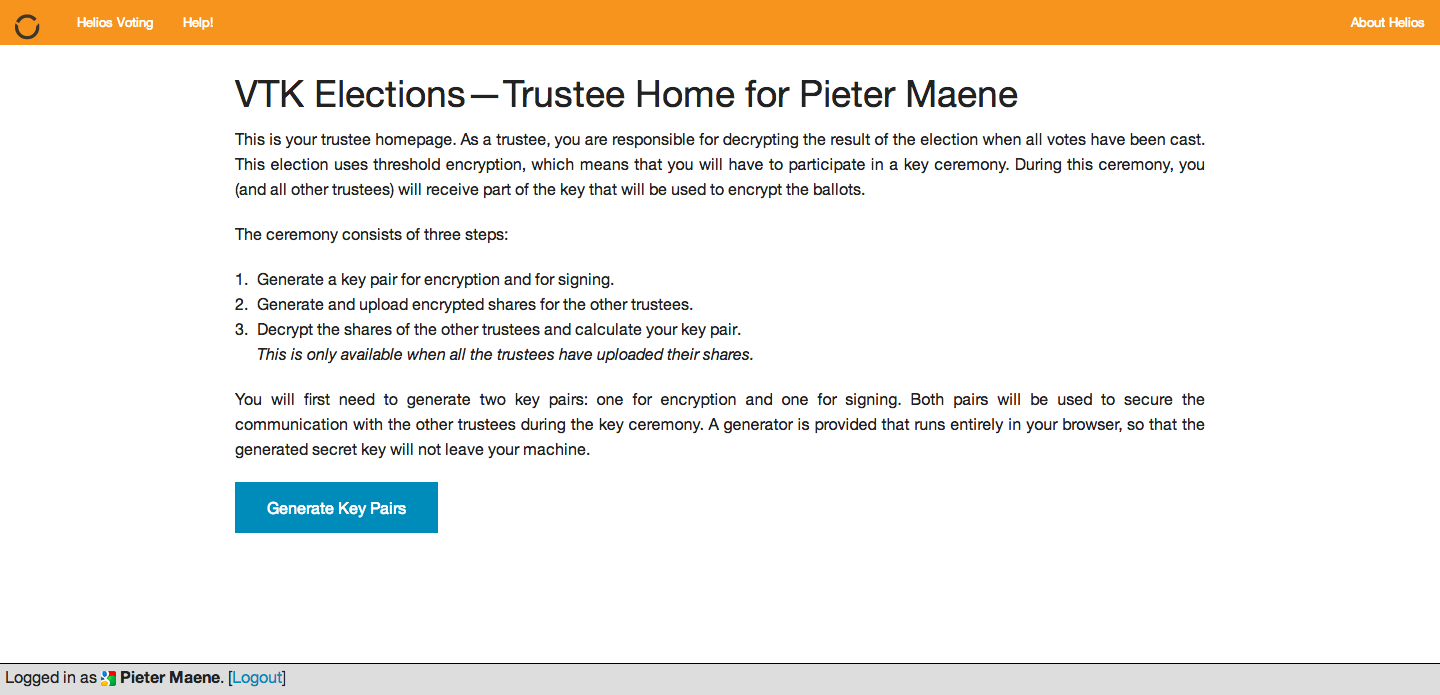
\includegraphics[width=\linewidth]{ui/trustees_home.png}}
  \caption{Trustee Dashboard}
  \label{fig:ui:trustees_home}
\end{figure}

\npar De trustee zal in totaal drie geheime sleutels genereren tijdens de sleutelceremonie (\ref{sec:proc:trustees}). Elke geheime sleutel moet lokaal bewaard worden in het JSON formaat. Oorspronkelijk moest de trustee deze zelf kopi\"eren naar een bestand. Om zijn sleutel te gebruiken, moest hij de inhoud daarvan opnieuw kopi\"eren naar een tekstvak.

\npar Door gebruik te maken van de HTML5 File API kon de omgang met de sleutels veel gebruiksvriendelijker gemaakt worden.\cite{ranganathan_sicking_file_api} Enerzijds voorziet deze API de \texttt{Blob} interface om lokaal bestanden te generen en aan te bieden als download in de browser. Anderzijds kan de \texttt{FileReader} interface gebruikt worden om objecten die voldoen aan de \texttt{Blob} of \texttt{File} interface uit te lezen. Een voorbeeld van deze laatste zijn bestanden die geselecteerd worden in een \texttt{file} input element.

\npar In het trustee dashboard wordt de eerste API interface gebruikt om de geheime sleutels onmiddelijk in een JSON bestand te plaatsen dat gedownload kan worden. Zo krijgen de trustees direct een bestand en worden de cryptografische details van de sleutel voor hen verborgen. De tweede interface wordt dan weer gebruikt om de trustee deze bestanden te laten selecteren om vervolgens de geheime sleutel uit te lezen naar het tekstvak. Het verschil tussen de oude en nieuwe manier van werken kan gezien worden in \ref{fig:ui:trustees_home_encrypted_shares_old} en \ref{fig:ui:trustees_home_encrypted_shares} respectievelijk.

\begin{figure}
  \center{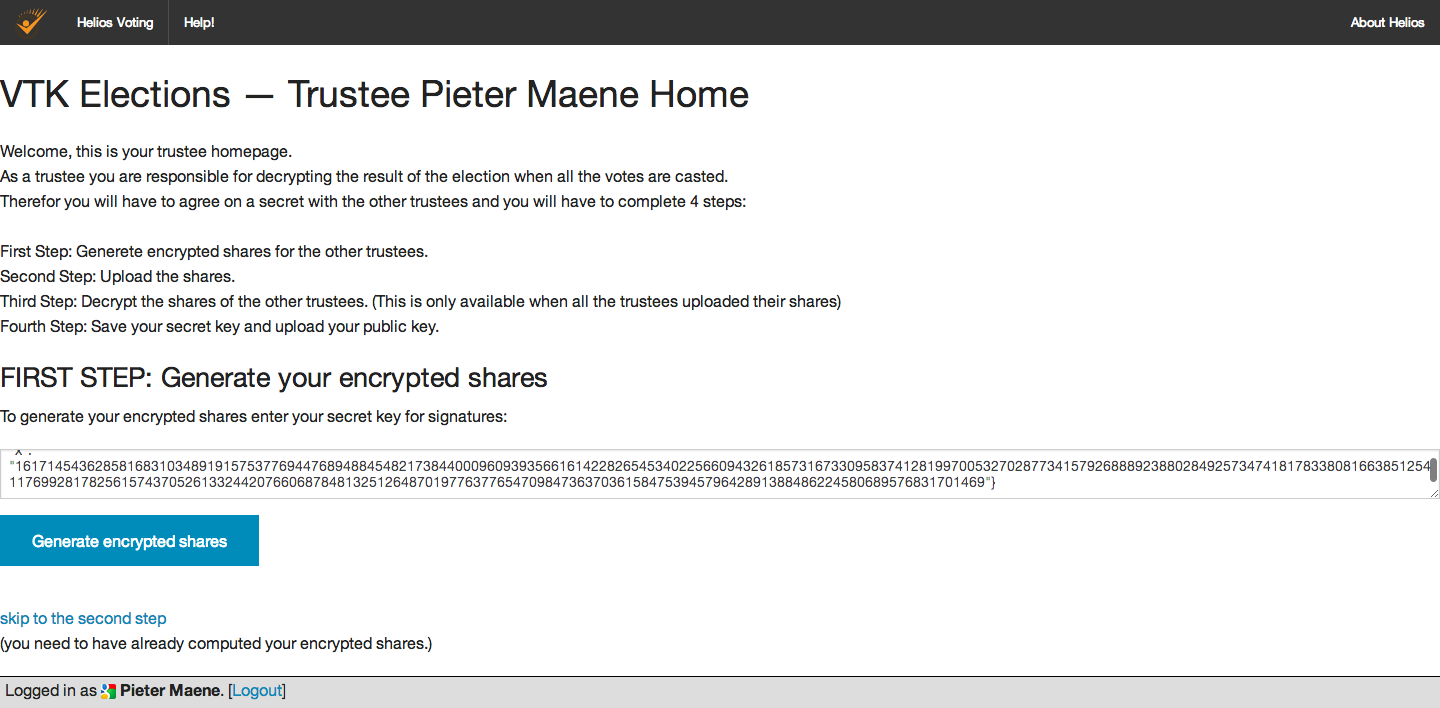
\includegraphics[width=\linewidth]{ui/trustees_home_encrypted_shares_old.png}}
  \caption{Genereren van encrypted shares (oud)}
  \label{fig:ui:trustees_home_encrypted_shares_old}
\end{figure}

\begin{figure}
  \center{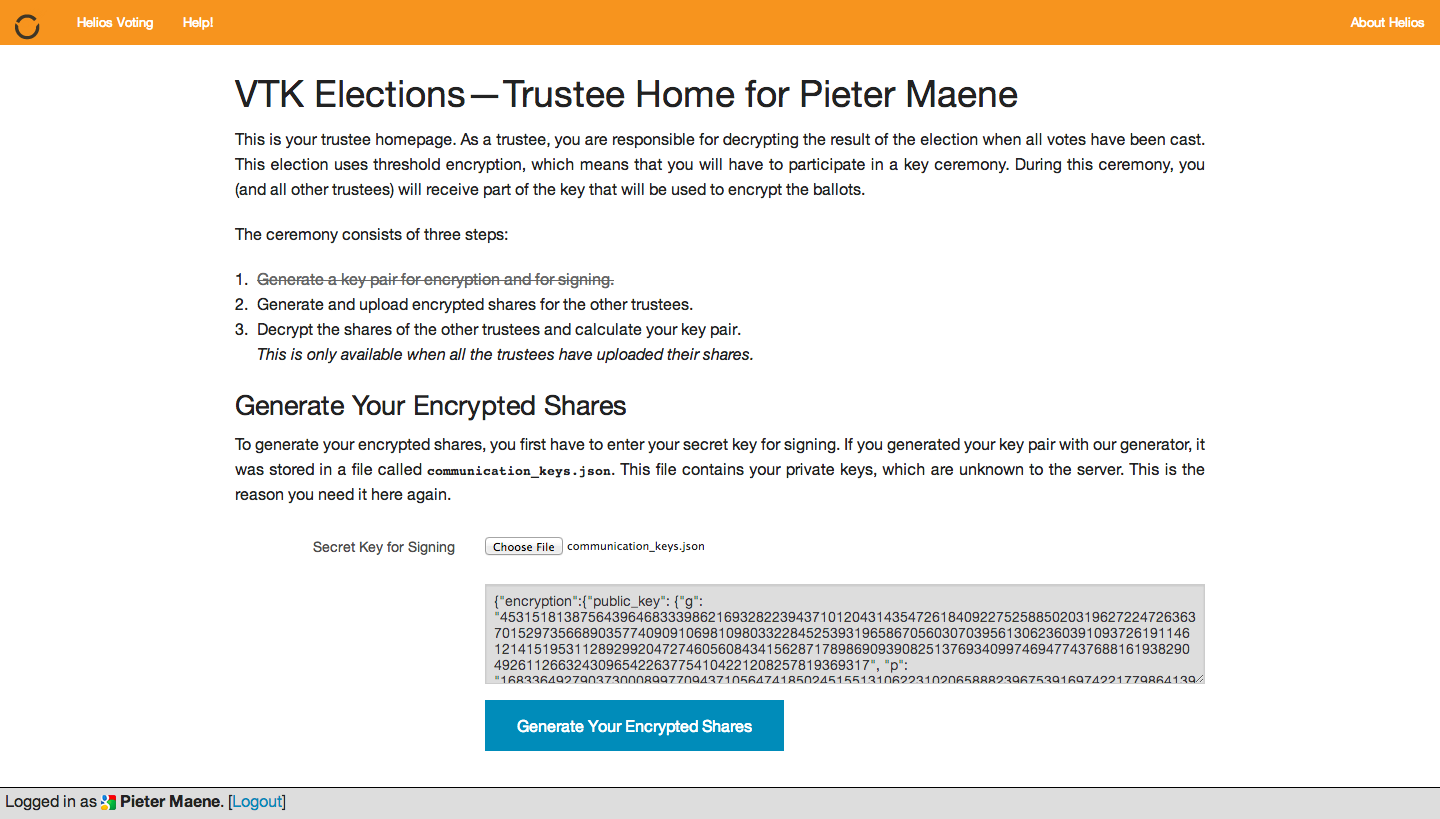
\includegraphics[width=\linewidth]{ui/trustees_home_encrypted_shares.png}}
  \caption{Genereren van encrypted shares}
  \label{fig:ui:trustees_home_encrypted_shares}
\end{figure}

\npar Om de communicatie te beveiligen worden twee sleutelparen gebruikt (\ref{sec:helios:communicatiesleutels}). Oorspronkelijk moesten deze apart gedownload worden. Omdat het voor de gebruiker eenvoudiger is om maar met \'e\'en bestand te moeten werken, werden deze samengevoegd.

\section{Controleapplicatie}
\label{sec:ui:controleapplicatie}

De controleapplicatie werd besproken in \ref{sec:helios:controleapplicatie}. Het resultaat van de verificatie werd oorspronkelijk onduidelijk weergegeven  (\ref{fig:ui:verifier_old}). Zoals gezien kan worden in \ref{fig:ui:verifier}, werd er meer structuur gebracht in de output.

\begin{figure}
  \center{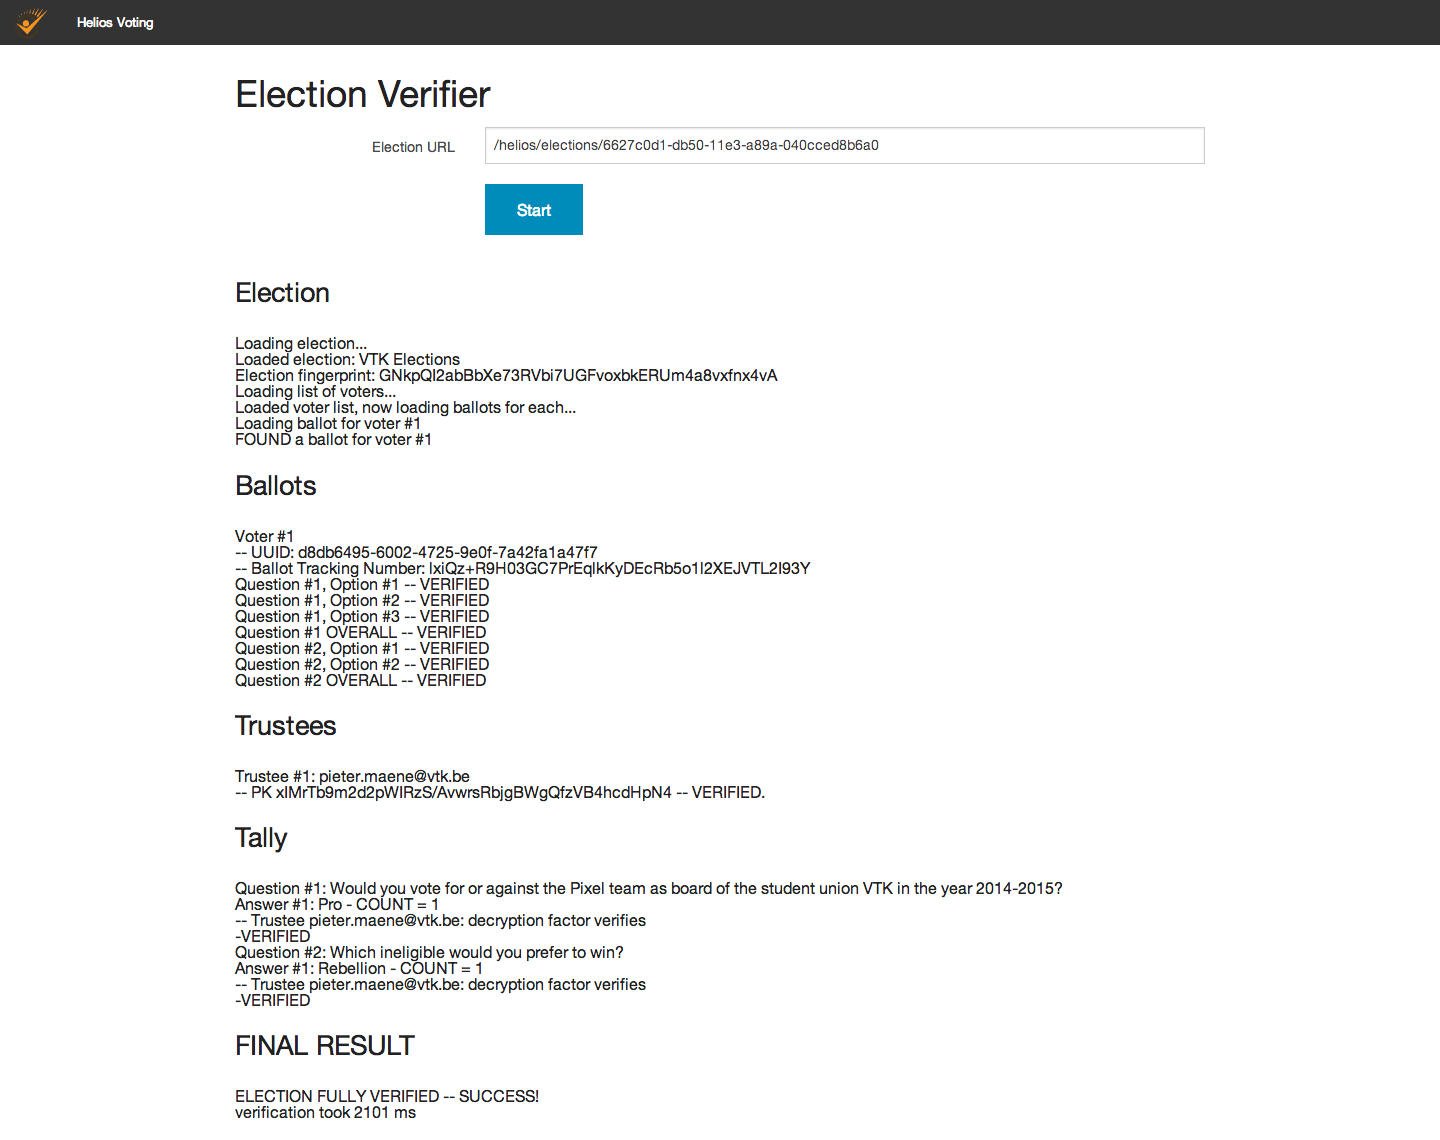
\includegraphics[width=\linewidth]{ui/verifier_old.png}}
  \caption{Controleapplicatie (oud)}
  \label{fig:ui:verifier_old}
\end{figure}

\begin{figure}
  \center{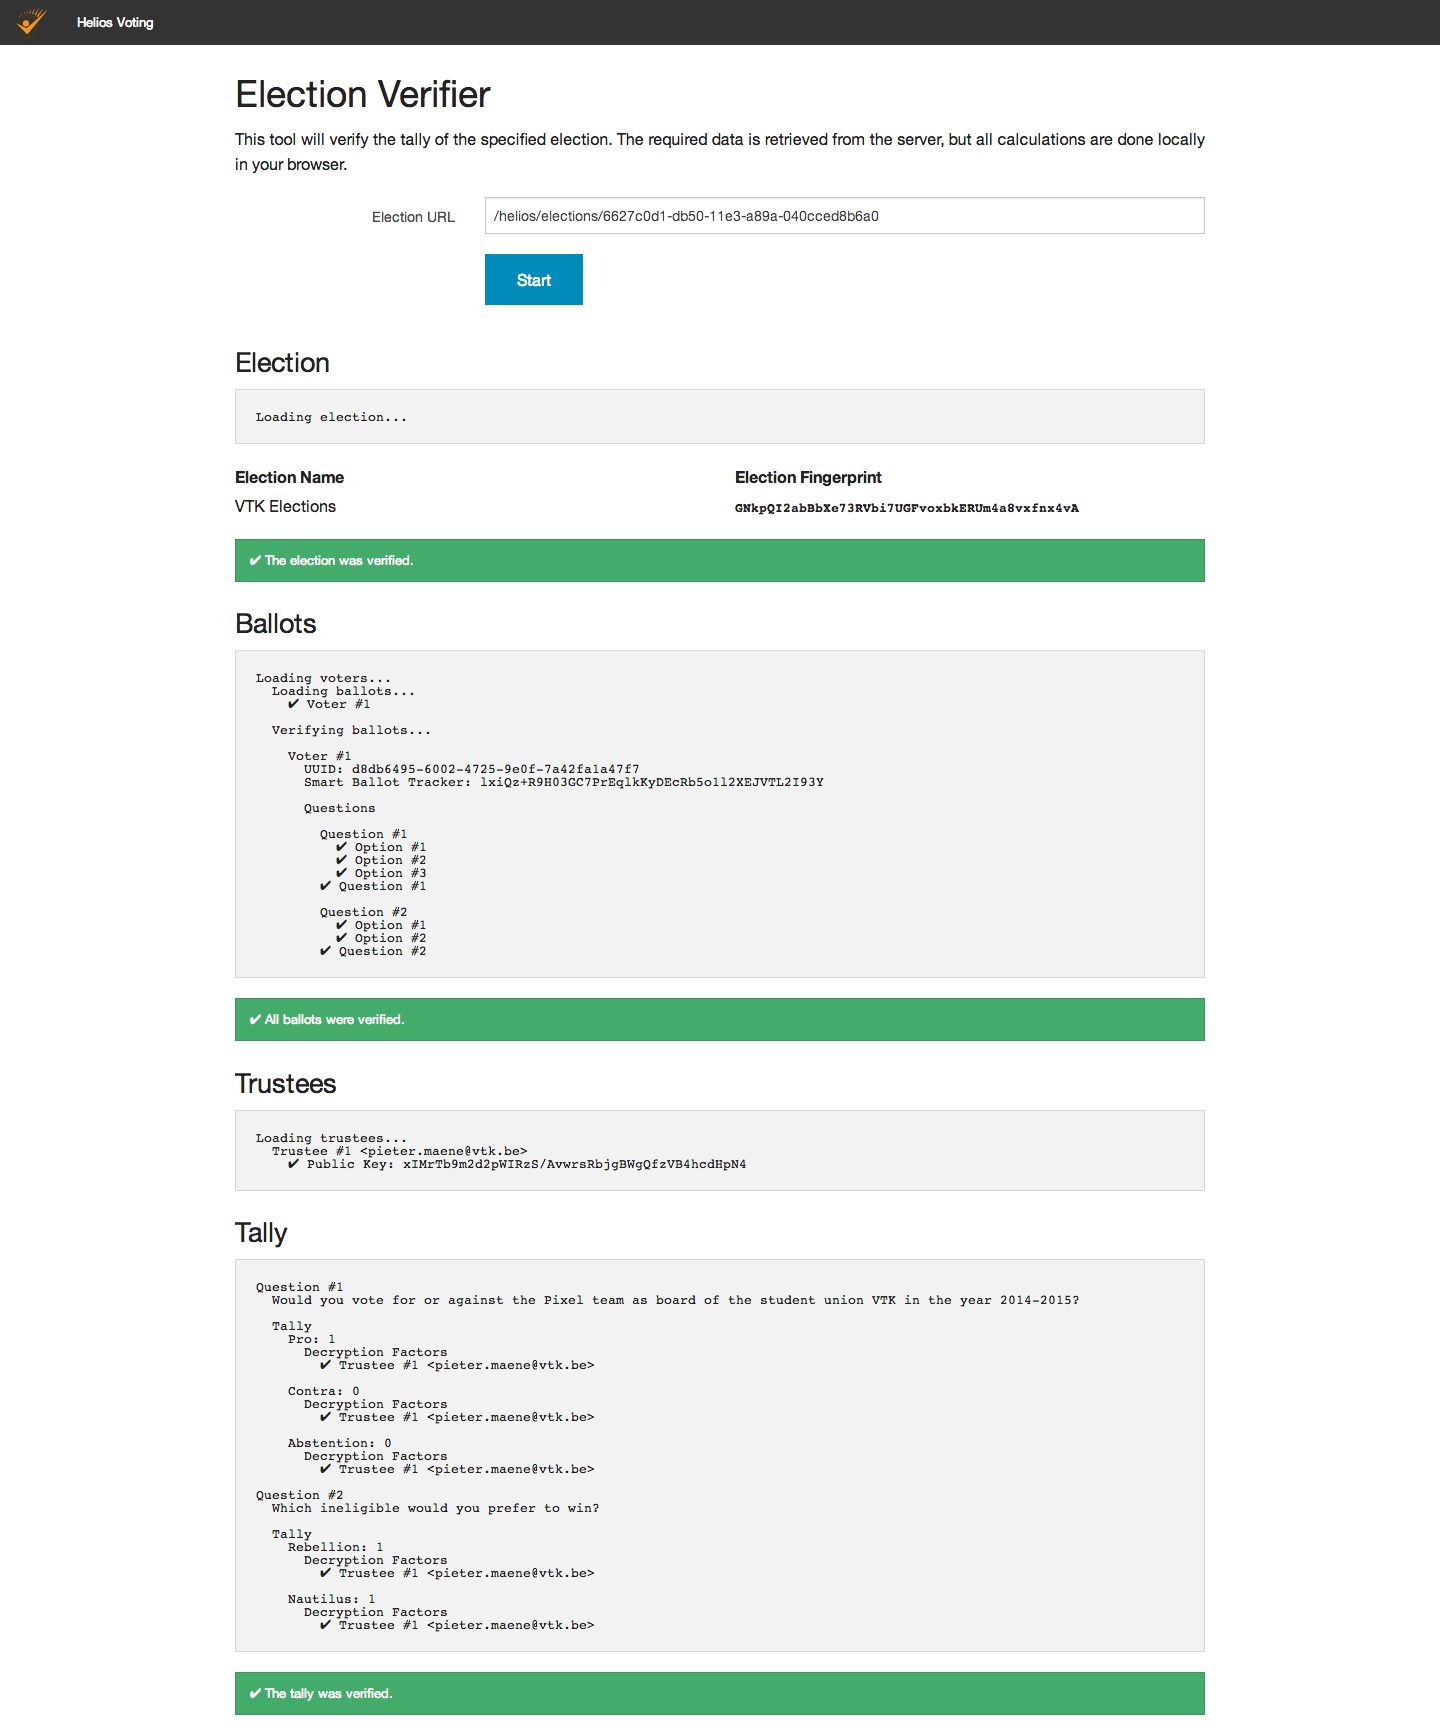
\includegraphics[width=\linewidth]{ui/verifier.png}}
  \caption{Controleapplicatie}
  \label{fig:ui:verifier}
\end{figure}
